\chapter{Specifikacija programske potpore}
		
	\section{Funkcionalni zahtjevi}
			
			\begin{comment}
			\textbf{\textit{dio 1. revizije}}\\
			
			\textit{Navesti \textbf{dionike} koji imaju \textbf{interes u ovom sustavu} ili  \textbf{su nositelji odgovornosti}. To su prije svega korisnici, ali i administratori sustava, naručitelji, razvojni tim.}\\
				
			\textit{Navesti \textbf{aktore} koji izravno \textbf{koriste} ili \textbf{komuniciraju sa sustavom}. Oni mogu imati inicijatorsku ulogu, tj. započinju određene procese u sustavu ili samo sudioničku ulogu, tj. obavljaju određeni posao. Za svakog aktora navesti funkcionalne zahtjeve koji se na njega odnose.}\\
			\end{comment}
			
			\noindent \textbf{Dionici:}
			
			\begin{packed_enum}
				
				\item Sportaš
				\item Trener
				\item Iznajmljivač
				\item Administrator
				\item Razvojni tim
				
			\end{packed_enum}
			
			\noindent \textbf{Aktori i njihovi funkcionalni zahtjevi:}
			
			
			\begin{packed_enum}
				
				\item  \underbar{Neregistrirani/neprijavljeni korisnik (inicijator) može:}
				
				\begin{packed_enum}
					
					\item koristiti tražilicu sportskih okupljanja/treninga
					\item pregledati na karti lokacije sportskih okupljanja/treninga
					\item odabrati sportsko okupljanje/trening i dobiti prikaz informacija o tom sportskom okupljanju/treningu (datum, vrijeme, mjesto, tip sporta)
					\item se registrirati u sustav kao sportaš, trener ili iznajmljivač, za što mu je potrebno ime, prezime, e-mail adresa i lozinka
					
				\end{packed_enum}
				
				
				\item  \underbar{Sportaš (inicijator) može:}
				
				\begin{packed_enum}
					
					\item se prijaviti u aplikaciju
					\item pregledavati i mijenjati osobne podatke
					\item se prijaviti za pojedino sportsko okupljanje/trening
					\item pristupiti kalendaru svih sportskih okupljanja/treninga na koje se prijavio ili koje je organizirao
					\item organizirati sportsko okupljanje za što su mu potrebni datum, vrijeme i mjesto okupljanja, tip sporta te maksimalan broj sudionika
					\item slati upit iznajmljivačima za iznajmljivanje sportskih površina/dvorana
					\item pregledavati sportska okupljanja/treninge predložene od strane aplikacije na temelju sportaševih osobnih podataka
					\item zatražiti da mu se dodijeli uloga trenera
					
				\end{packed_enum}
			
				\item  \underbar{Trener (inicijator) može:}
				
				\begin{packed_enum}
					
					\item se prijaviti u aplikaciju
					\item priložiti službenu dokumentaciju kojom potvrđuje da je trener za određene sportove
					\item pregledavati i mijenjati osobne podatke
					\item se prijaviti za pojedino sportsko okupljanje/trening
					\item slati upit iznajmljivačima za iznajmljivanje sportskih površina/dvorana
					\item organizirati sportska okupljanja za sve sportove i profesionalne (plaćene) treninge za one sportove za koje je potvrđen kao trener za što su mu potrebni datum, vrijeme, mjesto okupljanja, tip sporta te maksimalan broj sudionika
					\item pristupiti kalendaru u kojemu se nalaze sva sportska okupljanja kojima trener prisustvuje i svi njegovi termini treninga i podaci o tim treninzima
					\item koristiti tražilicu sportskih okupljanja/treninga
					
				\end{packed_enum}
			
				\item \underbar{Iznajmljivač (inicijator) može:}
			
				\begin{packed_enum}
				
					\item se prijaviti u aplikaciju
					\item pristupiti uređivaču sportskih objekata u kojemu može mijenjati podatke i termine za već dodane sportske objekte ili dodati novi objekt navodeći lokaciju, tip sportova koji se tamo mogu održavati, cijenu po satu, termine dostupne za rezervaciju i dokumentaciju kojom potvrđuje vlasništvo
					\item pristupiti kalendaru gdje su mu vidljivi svi odobreni termini za iznajmljivanje i novi termini koje su zatražili korisnici koje može odobriti ili odbaciti
					
				\end{packed_enum}
			
				\item \underbar{Administrator (inicijator) može:}
			
				\begin{packed_enum}
				
					\item se prijaviti u aplikaciju
					\item vidjeti sve registrirane korisnike i njihove podatke
					\item odobriti ili odbiti registracije trenera i iznajmljivača na temelju dokumentacije koju prilože
					\item korisnike dodavati, brisati ili im mijenjati razinu pristupa aplikaciji(sportaš, trener, iznajmljivač)
				
				\end{packed_enum}
			
				\item \underbar{Baza podataka (sudionik):}
				
				\begin{packed_enum}
					
					\item pohranjuje sve podatke o korisnicima i njihovim ovlastima
					\item pohranjuje sve podatke o sportskim okupljanjima i profesionalnim treninzima
					\item pohranjuje sve podatke o sportskim objektima koji su prijavljeni u aplikaciji
					
				\end{packed_enum}
			
			\end{packed_enum}
			
			\eject 
			
			
				
			\subsection{Obrasci uporabe}
				
				%\textbf{\textit{dio 1. revizije}}
				
				\subsubsection{Opis obrazaca uporabe}
					\begin{comment}
					\textit{Funkcionalne zahtjeve razraditi u obliku obrazaca uporabe. Svaki obrazac je potrebno razraditi prema donjem predlošku. Ukoliko u nekom koraku može doći do odstupanja, potrebno je to odstupanje opisati i po mogućnosti ponuditi rješenje kojim bi se tijek obrasca vratio na osnovni tijek.}\\
					\end{comment}

					\noindent \underbar{\textbf{UC1 -Pregled sportskih aktivnosti}}
					\begin{packed_item}
						
						\item \textbf{Glavni sudionik: }Korisnik
						\item  \textbf{Cilj:} Pregledati dostupna sportska okupljanja i treninge
						\item  \textbf{Sudionici:} Baza podataka
						\item  \textbf{Preduvjet:} -
						\item  \textbf{Opis osnovnog tijeka:}
						
						\item[] \begin{packed_enum}
							
							\item Karta i tražilica su prikazani prilikom učitavanja aplikacije
							\item Korisnik na karti odabire sportsko okupljanje ili trening
							\item Prikazuju se informacije o odabranom sportskom okupljanju/treningu
						\end{packed_enum}
						
					\end{packed_item}
					
					\noindent \underbar{\textbf{UC2 - Pretraživanje sportskih aktivnosti}}
					\begin{packed_item}
						
						\item \textbf{Glavni sudionik: }Korisnik
						\item  \textbf{Cilj:} Pretraživati dostupna sportska okupljanja i treninge
						\item  \textbf{Sudionici:} Baza podataka
						\item  \textbf{Preduvjet:} -
						\item  \textbf{Opis osnovnog tijeka:}
						
						\item[] \begin{packed_enum}
							
							\item Karta i tražilica su prikazani prilikom učitavanja aplikacije
							\item Korisnik u tražilicu upisuje parametre (mjesto, vrijeme, sport)
							\item Karta se ažurira na temelju unesenih parametara
						\end{packed_enum}
						
					\end{packed_item}
					
					\noindent \underbar{\textbf{UC3 - Registracija}}
					\begin{packed_item}
						
						\item \textbf{Glavni sudionik: }Korisnik
						\item  \textbf{Cilj:} Stvoriti korisnički račun za pristup sustavu
						\item  \textbf{Sudionici:} Baza podataka
						\item  \textbf{Preduvjet:} -
						\item  \textbf{Opis osnovnog tijeka:}
						
						\item[] \begin{packed_enum}
							
							\item Korisnik odabire opciju za registraciju
							\item Korisnik unosi tražene podatke
							\item Korisnik prima obavijest o uspješnoj registraciji
						\end{packed_enum}
						
						\item  \textbf{Opis mogućih odstupanja:}
						
						\item[] \begin{packed_item}
							
							\item[2.a] Odabir već zauzete e-mail adrese, upis podataka u nedozvoljenom formatu, upis neispravne e-mail adrese 
							\item[] \begin{packed_enum}
								
								\item Sustav obavještava korisnika o neuspjeloj registraciji i vraća ga na stranicu za registraciju
								\item Korisnik mijenja neispravno upisane podatke ili odustaje od registracije
								
							\end{packed_enum}
							
						\end{packed_item}
					\end{packed_item}
					
					\noindent \underbar{\textbf{UC4 - Prijava u sustav}}
					\begin{packed_item}
						
						\item \textbf{Glavni sudionik: }Korisnik
						\item  \textbf{Cilj:} Dobiti pristup korisničkom sučelju 
						\item  \textbf{Sudionici:} Baza podataka
						\item  \textbf{Preduvjet:} Registracija
						\item  \textbf{Opis osnovnog tijeka:}
						
						\item[] \begin{packed_enum}
							
							\item Korisnik odabire opciju za prijavu
							\item Korisnik unosi e-mail adresu i lozinku
							\item Potvrda o ispravnosti unesenih podataka
							\item Pristup korisničkim funkcijama
						\end{packed_enum}
						
						\item  \textbf{Opis mogućih odstupanja:}
						
						\item[] \begin{packed_item}
							
							\item[2.a] Neispravna e-mail adresa ili lozinka
							\item[] \begin{packed_enum}
								
								\item Sustav obavještava korisnika o neuspjeloj prijavi i vraća ga na stranicu za prijavu
								\item Korisnik mijenja neispravno unesene podatke ili odustaje od prijave
								
							\end{packed_enum}
							
						\end{packed_item}
					\end{packed_item}
					
					\noindent \underbar{\textbf{UC5 -Pregled osobnih podataka}}
					\begin{packed_item}
						
						\item \textbf{Glavni sudionik: }Sportaš
						\item  \textbf{Cilj:} Pregledati osobne podatke
						\item  \textbf{Sudionici:} Baza podataka
						\item  \textbf{Preduvjet:} Korisnik je prijavljen
						\item  \textbf{Opis osnovnog tijeka:}
						
						\item[] \begin{packed_enum}
							
							\item Korisnik odabire opciju "Osobni podatci"
							\item Prikazuju se osobni podatci korisnika
						\end{packed_enum}
						
					\end{packed_item}
					
					\noindent \underbar{\textbf{UC6 -Promjena osobnih podataka}}
					\begin{packed_item}
						
						\item \textbf{Glavni sudionik: }Sportaš
						\item  \textbf{Cilj:} Promijeniti  osobne podatke
						\item  \textbf{Sudionici:} Baza podataka
						\item  \textbf{Preduvjet:} Korisnik je prijavljen i odabrao je opciju "Osobni podatci"
						\item  \textbf{Opis osnovnog tijeka:}
						
						\item[] \begin{packed_enum}
							
							\item Korisnik odabire opciju za promjenu osobnih podataka
							\item Korisnik mijenja osobne podatke
							\item Korisnik sprema promjene
						\end{packed_enum}
						
					\end{packed_item}
					
					\noindent \underbar{\textbf{UC7 -Prijava na sportsku aktivnost}}
					\begin{packed_item}
						
						\item \textbf{Glavni sudionik: }Sportaš
						\item  \textbf{Cilj:} Prijaviti se na sportsko okupljanje ili trening
						\item  \textbf{Sudionici:} Baza podataka
						\item  \textbf{Preduvjet:} Korisnik je prijavljen
						\item  \textbf{Opis osnovnog tijeka:}
						
						\item[] \begin{packed_enum}
							
							\item Korisnik odabire sportsku aktivnost na koju se želi prijaviti
							\item Korisnik odabire opciju "Prijavi se"
							\item Korisnik potvrdi da se želi prijaviti za odabranu sportsku aktivnost
						\end{packed_enum}
						
					\end{packed_item}
					
					\noindent \underbar{\textbf{UC8 -Pregled prijavljenih sportskih aktivnosti}}
					\begin{packed_item}
						
						\item \textbf{Glavni sudionik: }Sportaš
						\item  \textbf{Cilj:} Pregledati sportska okupljanja ili treninge na koje se korisnik prijavio ili koje je organizirao
						\item  \textbf{Sudionici:} Baza podataka
						\item  \textbf{Preduvjet:} Korisnik je prijavljen
						\item  \textbf{Opis osnovnog tijeka:}
						
						\item[] \begin{packed_enum}
							
							\item Korisnik odabire opciju "Moje prijave"
							\item Prikazuje se kalendar s upisanim terminima svih prijavljenih ili organiziranih sportskih aktivnosti
						\end{packed_enum}
						
					\end{packed_item}
					
					\noindent \underbar{\textbf{UC9 -Organiziranje sportskog okupljanja}}
					\begin{packed_item}
						
						\item \textbf{Glavni sudionik: }Sportaš
						\item  \textbf{Cilj:} Organizirati sportsko okupljanje
						\item  \textbf{Sudionici:} Baza podataka
						\item  \textbf{Preduvjet:} Korisnik je prijavljen
						\item  \textbf{Opis osnovnog tijeka:}
						
						\item[] \begin{packed_enum}
							
							\item Korisnik odabire opciju "Organiziraj sportsko okupljanja"
							\item Korisnik upisuje tražene podatke
							\item Korisnik potvrđuje unesene podatke
							\item Korisnika se preusmjerava na stranicu za pregled prijavljenih sportskih aktivnosti
						\end{packed_enum}
						
						\item  \textbf{Opis mogućih odstupanja:}
						
						\item[] \begin{packed_item}
							
							\item[2.a] Upisano mjesto sportskog okupljanja nije javno i korisnik ga nije iznajmio
							\item[] \begin{packed_enum}
								
								\item Sustav obavještava korisnika da nije iznajmio sportsku površinu/dvoranu te mu daje opciju za iznajmljivanje
								\item Korisnik može promijeniti tražene podatke, odabrati opciju za iznajmljivanje ili odustati od organizacije
								
							\end{packed_enum}
							
						\end{packed_item}
					\end{packed_item}
					
					\noindent \underbar{\textbf{UC10 -Iznajmljivanje sportskih površina/dvorana}}
					\begin{packed_item}
						
						\item \textbf{Glavni sudionik: }Sportaš
						\item  \textbf{Cilj:} Iznajmljivanje sportske površine ili dvorane
						\item  \textbf{Sudionici:} Baza podataka
						\item  \textbf{Preduvjet:} Korisnik je prijavljen i odabrao je opciju "Organiziraj sportsko okupljanje"
						\item  \textbf{Opis osnovnog tijeka:}
						
						\item[] \begin{packed_enum}
							
							\item Korisnik odabire opciju "Iznajmljivanje sportske površine ili dvorane"
							\item Korisnik odabire sportsku površinu ili dvoranu koju želi iznajmiti
							\item Korisnik odabire datum kada želi iznajmiti odabranu sportsku površinu ili dvoranu
							\item Korisniku se prikazuju slobodni termini za odabrani datum
							\item Korisnik odabire željeno vrijeme
							\item Korisnik odabire opciju "Potvrdi rezervaciju"
						\end{packed_enum}
						
						\item  \textbf{Opis mogućih odstupanja:}
						
						\item[] \begin{packed_item}
							
							\item[3.a] Za odabrani datum nema slobodnih termina 
							\item[] \begin{packed_enum}
								
								\item Sustav javlja korisniku da za odabrani datum nema slobodnih termina i daje mu opciju promjene datuma
								
							\end{packed_enum}
							
						\end{packed_item}
						
					\end{packed_item}
					
					\noindent \underbar{\textbf{UC11 -Pregled predloženih aktivnosti }}
					\begin{packed_item}
						
						\item \textbf{Glavni sudionik: }Sportaš
						\item  \textbf{Cilj:} Pregled sportskih aktivnosti predloženih od strane sustava
						\item  \textbf{Sudionici:} Baza podataka
						\item  \textbf{Preduvjet:} Korisnik je prijavljen
						\item  \textbf{Opis osnovnog tijeka:}
						
						\item[] \begin{packed_enum}
							
							\item Korisnik odabire opciju "Predloži za mene"
							\item Sustav prikazuje predložena sportska okupljanja i treninge na temelju osobnih podataka korisnika
							
						\end{packed_enum}
						
					\end{packed_item}
					
					
					
					\noindent \underbar{\textbf{UC12 - Dodavanje sportskog objekta}}
					\begin{packed_item}
						
						\item \textbf{Glavni sudionik: } Iznajmljivač
						\item  \textbf{Cilj:} Dodati novi sportski objekt
						\item  \textbf{Sudionici:} Baza podataka, administrator
						\item  \textbf{Preduvjet:} Korisnik je prijavljen s ovlastima iznajmljivača 
						\item  \textbf{Opis osnovnog tijeka:}
						
						\item[] \begin{packed_enum}
							
							\item Iznajmljivač odabire opciju "Dodaj novi sportski objekt"
							\item Iznajmljivač ispunjava podatke za objekt i prilaže dokumentaciju o vlasništvu
							\item Administrator pregledava i potvrđuje dokumentaciju
							\item Iznajmljivaču se prikazuje poruka o uspješnom dodavanju objekta
							
						\end{packed_enum}
						
						\item  \textbf{Opis mogućih odstupanja:}
						
						\item[] \begin{packed_item}
							
							\item[3.a] Administrator odbija dodavanje objekta zbog nevažeće dokumentacije
							\item[] \begin{packed_enum}
								
								\item Sustav obavještava iznajmljivača o neuspješnom dodavanju objekta
								\item Iznajmljivač može odustati ili ponovno dodati objekt s važećom dokumentacijom
								
							\end{packed_enum}
							
						\end{packed_item}
					
					\end{packed_item}
				
				
				
					\noindent \underbar{\textbf{UC13 - Pregled sportskog objekta}}
					\begin{packed_item}
						
						\item \textbf{Glavni sudionik: } Iznajmljivač
						\item  \textbf{Cilj:}  Pregledati podatke i slobodne termine za sportski objekt
						\item  \textbf{Sudionici:} Baza podataka
						\item  \textbf{Preduvjet:} Korisnik je prijavljen s ovlastima iznajmljivača, administrator mu je odobrio prijavu tog sportskog objekta
						\item  \textbf{Opis osnovnog tijeka:}
						
						\item[] \begin{packed_enum}
							
							\item Iznajmljivač odabire objekt za koji želi pregledati podatke
							\item Prikazuju se podaci i slobodni termini za taj sportski objekt
							
						\end{packed_enum}
						
					\end{packed_item}
					
					
					\noindent \underbar{\textbf{UC14 - Uređivanje sportskog objekta}}
					\begin{packed_item}
						
						\item \textbf{Glavni sudionik: } Iznajmljivač
						\item  \textbf{Cilj:}  Urediti podatke za sportski objekt
						\item  \textbf{Sudionici:} Baza podataka
						\item  \textbf{Preduvjet:} Korisnik je prijavljen s ovlastima iznajmljivača te pregledava podatke i slobodne termine za odabrani sportski objekt.
						\item  \textbf{Opis osnovnog tijeka:}
						
						\item[] \begin{packed_enum}
							
							\item Iznajmljivač odabire "Uredi"
							\item Iznajmljivač mijenja podatke ili slobodne termine za taj objekt
							\item Iznajmljivač odabire opciju "Spremi"
							\item Promjene se spremaju u bazu podataka
							
						\end{packed_enum}
						
						\item  \textbf{Opis mogućih odstupanja:}
						
						\item[] \begin{packed_item}
							
							\item[2.a] Iznajmljivač promjeni podatke, ali ne odabere opciju "Spremi"
							\item[] \begin{packed_enum}
								
								\item Sustav obavještava iznajmljivača da nije spremio podatke prije izlaska iz prozora
							
							\end{packed_enum}
							
						\end{packed_item}
						
					\end{packed_item}
				
					
					\noindent \underbar{\textbf{UC15 - Pregled rezervacija sportskog objekta}}
					\begin{packed_item}
						
						\item \textbf{Glavni sudionik: } Iznajmljivač
						\item  \textbf{Cilj:}  Odobriti nove termine koje su korisnici zatražili i vidjeti već odobrene termine
						\item  \textbf{Sudionici:} Baza podataka
						\item  \textbf{Preduvjet:} Korisnik je prijavljen s ovlastima iznajmljivača 
						\item  \textbf{Opis osnovnog tijeka:}
						
						\item[] \begin{packed_enum}
							
							\item Iznajmljivač odabire kalendar
							\item Iznajmljivač vidi datume s već odobrenim terminima te listu zahtjeva za iznajmljivanjem
							\item Za svaki zahtjev može odabrati "Potvrdi" ili "Odbaci"
							
						\end{packed_enum}
						
					\end{packed_item}
				
				
					\noindent \underbar{\textbf{UC16 - Pregled korisnika}}
					\begin{packed_item}
						
						\item \textbf{Glavni sudionik: } Administrator
						\item  \textbf{Cilj:}  Pregledati registrirane korisnike
						\item  \textbf{Sudionici:} Baza podataka
						\item  \textbf{Preduvjet:} Korisnik je prijavljen s ovlastima administratora 
						\item  \textbf{Opis osnovnog tijeka:}
						
						\item[] \begin{packed_enum}
							
							\item Administrator odabire opciju pregledavanja registriranih korisnika
							\item Sustav prikazuje listu registriranih korisnika
							
						\end{packed_enum}
					
					\end{packed_item}
				
					\noindent \underbar{\textbf{UC17 - Brisanje korisnika}}
					\begin{packed_item}
					
						\item \textbf{Glavni sudionik: } Administrator
						\item  \textbf{Cilj:}  Obrisati registriranog korisnika
						\item  \textbf{Sudionici:} Baza podataka
						\item  \textbf{Preduvjet:} Korisnik je prijavljen s ovlastima administratora i odabrao je opciju pregleda registriranih korisnika
						\item  \textbf{Opis osnovnog tijeka:}
					
						\item[] \begin{packed_enum}
						
							\item Administrator iz liste bira korisnika kojeg želi izbrisati
							\item Odabirom opcije "Obriši" briše se korisnik te sve njegove prijave na sportske aktivnosti, njegovi sportski objekti te svi treninzi koje je organizirao
						
						\end{packed_enum}
					
					\end{packed_item}
				
						\noindent \underbar{\textbf{UC18 - Promjena prava pristupa}}
					\begin{packed_item}
						
						\item \textbf{Glavni sudionik: } Administrator
						\item  \textbf{Cilj:}  Promijeniti prava pristupa registriranom korisniku
						\item  \textbf{Sudionici:} Baza podataka
						\item  \textbf{Preduvjet:} Korisnik je prijavljen s ovlastima administratora i odabrao je opciju pregleda registriranih korisnika
						\item  \textbf{Opis osnovnog tijeka:}
						
						\item[] \begin{packed_enum}
							
							\item Administrator iz liste bira korisnika kojemu želi promijeniti ovlasti
							\item Administrator bira koju razinu ovlasti daje odabranom korisniku
							
						\end{packed_enum}
						
					\end{packed_item}
			
						\noindent \underbar{\textbf{UC19 - Pregled zahtjeva }}
					\begin{packed_item}
						
						\item \textbf{Glavni sudionik: } Administrator
						\item  \textbf{Cilj:}  Odobriti ili odbaciti zahtjeve za registraciju trenera i zahtjeve iznajmljivača za dodavanje sportskog objekta
						\item  \textbf{Sudionici:} Baza podataka
						\item  \textbf{Preduvjet:} Korisnik je prijavljen s ovlastima administratora 
						\item  \textbf{Opis osnovnog tijeka:}
						
						\item[] \begin{packed_enum}
							
							\item Administrator odabire opciju pregledavanja zahtjeva
							\item Administrator uz svaki zahtjev ima opciju dohvaćanja priložene dokumentacije
							\item Administrator nakon pregleda dokumentacije zahtjeva bira "Potvrdi" ili "Odbaci"
							
						\end{packed_enum}
						
					\end{packed_item}
					
					\noindent \underbar{\textbf{UC20 -Organiziranje profesionalnog treninga}}
					\begin{packed_item}
						
						\item \textbf{Glavni sudionik: }Trener
						\item  \textbf{Cilj:} Organizirati profesionalni trening
						\item  \textbf{Sudionici:} Baza podataka
						\item  \textbf{Preduvjet:} Korisnik je prijavljen i odobrena mu je licenca trenera za određeni sport
						\item  \textbf{Opis osnovnog tijeka:}
						
						\item[] \begin{packed_enum}
							
							\item Korisnik odabire opciju "Organiziraj profesionalni trening"
							\item Korisnik upisuje tražene podatke
							\item Korisnik potvrđuje upisane podatke
							\item Korisnika se preusmjerava na stranicu za pregled prijavljenih sportskih aktivnosti
							
						\end{packed_enum}
						
						\item  \textbf{Opis mogućih odstupanja:}
						
						\item[] \begin{packed_item}
							
							\item[2.a] Upisano mjesto profesionalnog treninga nije javno i korisnik ga nije iznajmio
							\item[] \begin{packed_enum}
								
								\item Sustav obavještava korisnika da nije iznajmio sportsku površinu/dvoranu te mu daje opciju za iznajmljivanje
								\item Korisnik može promijeniti tražene podatke, odabrati opciju za iznajmljivanje ili odustati od organizacije
								
							\end{packed_enum}
							
						\end{packed_item}
					\end{packed_item}
					
					\noindent \underbar{\textbf{UC21 -Prilaganje službene dokumentacije}}
					\begin{packed_item}
						
						\item \textbf{Glavni sudionik: }Sportaš
						\item  \textbf{Cilj:} Dobiti odgovarajuću ulogu i odgovarajuće ovlasti
						\item  \textbf{Sudionici:} Baza podataka, Administrator
						\item  \textbf{Preduvjet:} Korisnik je prijavljen
						\item  \textbf{Opis osnovnog tijeka:}
						
						\item[] \begin{packed_enum}
							
							\item Korisnik odabire opciju "Dodaj službenu dokumentaciju"
							\item Korisnik upisuje tražene podatke
							\item Korisnik potvrđuje upisane podatke
							\item Administrator zaprima prijavu
							\item Korisnika se preusmjerava na stranicu kojom se korisniku daje do znanja da je njegova prijava zaprimljena te da će biti obaviješten kada ona bude obrađena
							
						\end{packed_enum}
						
					\end{packed_item}
					
%					\noindent \underbar{\textbf{UC$<$broj obrasca$>$ -$<$ime obrasca$>$}}
%					\begin{packed_item}
%						
%						\item \textbf{Glavni sudionik: }$<$sudionik$>$
%						\item  \textbf{Cilj:} $<$cilj$>$
%						\item  \textbf{Sudionici:} $<$sudionici$>$
%						\item  \textbf{Preduvjet:} $<$preduvjet$>$
%						\item  \textbf{Opis osnovnog tijeka:}
						
%						\item[] \begin{packed_enum}
							
%							\item $<$opis korak jedan$>$
%							\item $<$opis korak dva$>$
%							\item $<$opis korak tri$>$
%							\item $<$opis korak četiri$>$
%						\end{packed_enum}
						
%						\item  \textbf{Opis mogućih odstupanja:}
						
%						\item[] \begin{packed_item}
							
%							\item[2.a] $<$opis mogućeg scenarija odstupanja u koraku 2$>$
%							\item[] \begin{packed_enum}
								
%								\item $<$opis rješenja mogućeg scenarija korak 1$>$
%							\item $<$opis rješenja mogućeg scenarija korak 2$>$
								
							%\end{packed_enum}
							%\item[2.b] $<$opis mogućeg scenarija odstupanja u koraku 2$>$
							%\item[3.a] $<$opis mogućeg scenarija odstupanja  u koraku 3$>$
%							
%						\end{packed_item}
%					\end{packed_item}
				
					
				\subsubsection{Dijagrami obrazaca uporabe}
					
					%\textit{Prikazati odnos aktora i obrazaca uporabe odgovarajućim UML dijagramom. Nije nužno nacrtati sve na jednom dijagramu. Modelirati po razinama apstrakcije i skupovima srodnih funkcionalnosti.}
					\begin{figure}[H]
						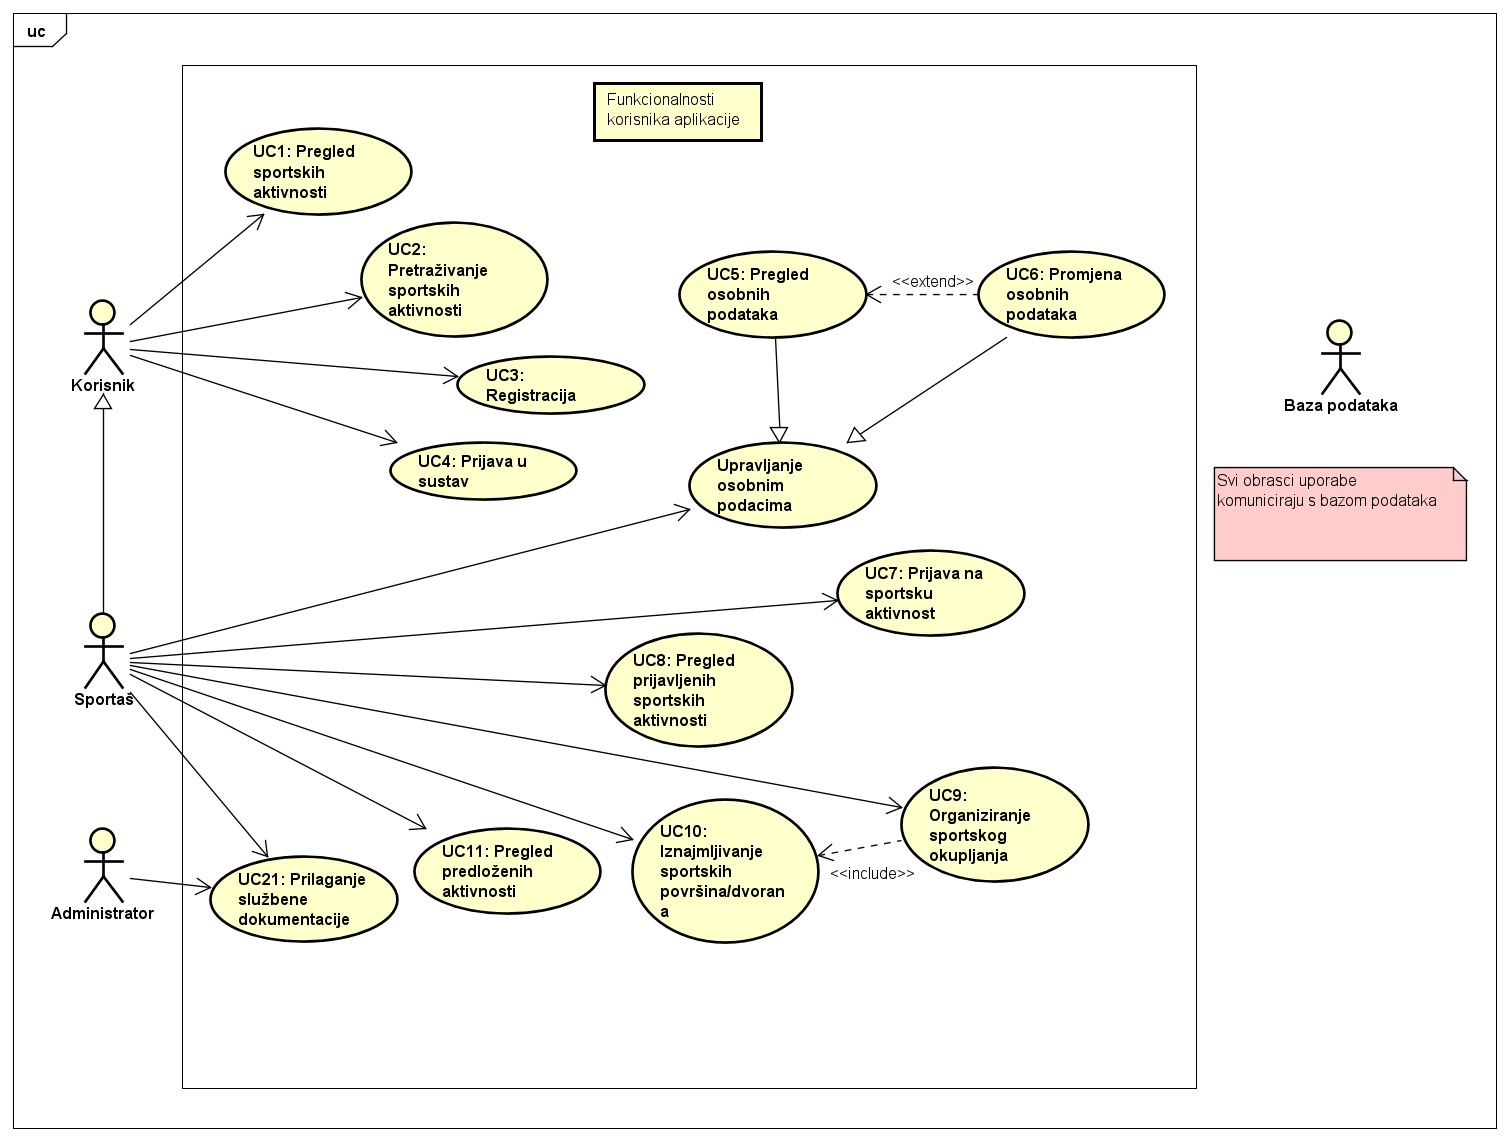
\includegraphics[width=1\linewidth]{slike/KorisnikSportas.PNG}
						\centering
						\caption{Funkcionalnosti korisnika aplikacije}
						\label{fig:funkcionalnosti_korisnik}
					\end{figure}
					\begin{figure}[H]
						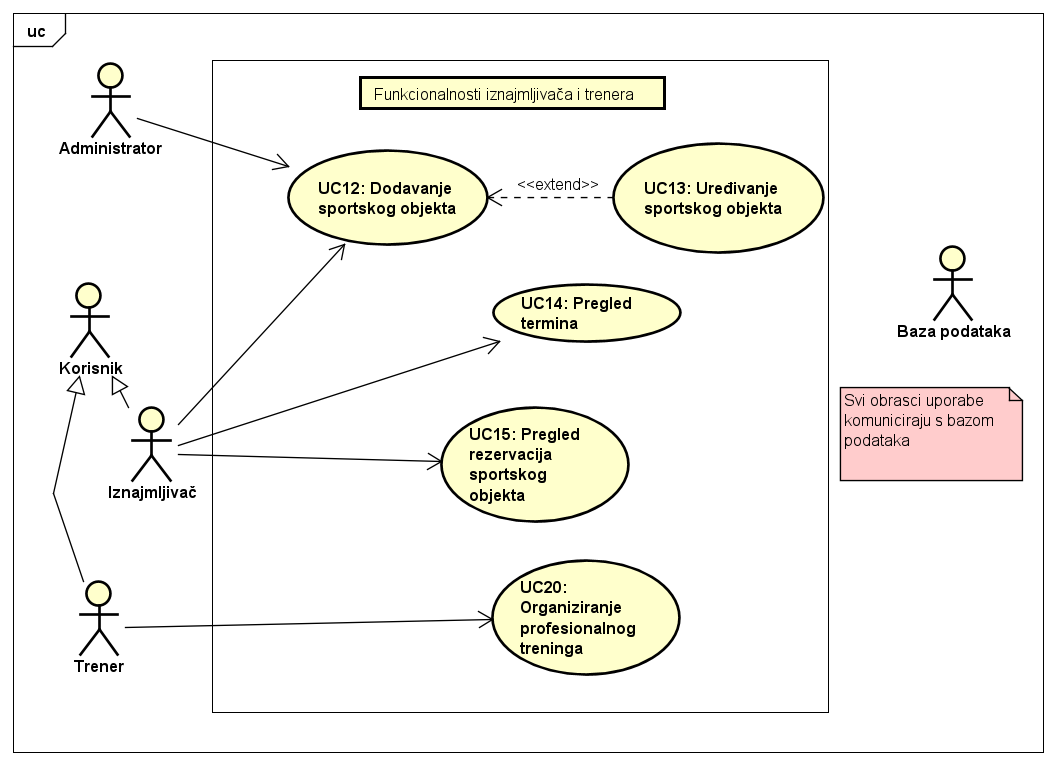
\includegraphics[width=1\linewidth]{slike/IznajmljivacTrener.PNG}
						\centering
						\caption{Funkcionalnosti iznajmljivača i trenera}
						\label{fig:funkcionalnosti_iznajmljivac_trener}
					\end{figure}
					\begin{figure}[H]
						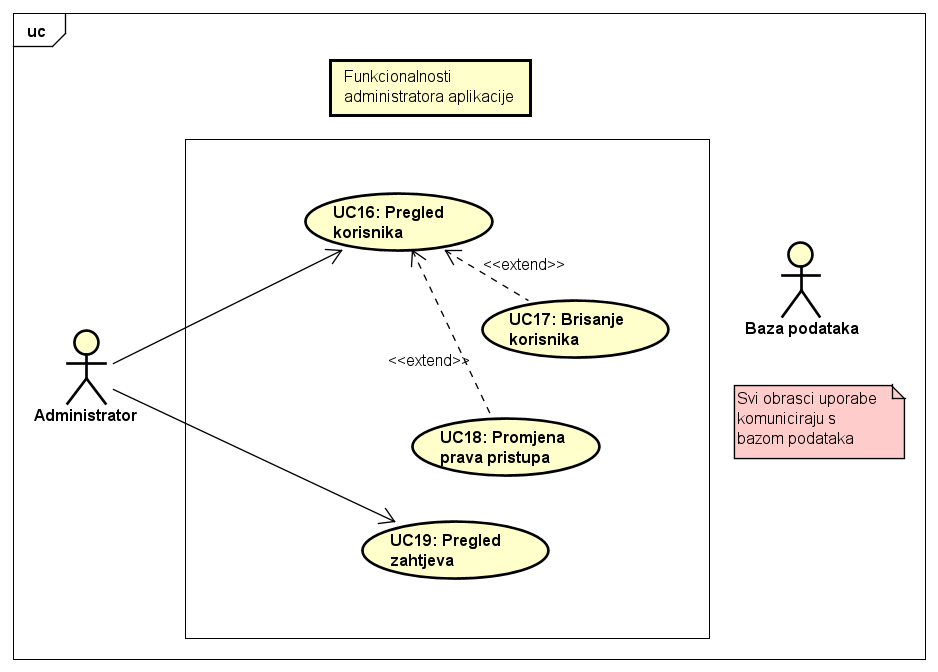
\includegraphics[width=1\linewidth]{slike/Administrator.PNG}
						\centering
						\caption{Funkcionalnosti administratora aplikacije}
						\label{fig:funkcionalnosti_administrator}
					\end{figure}
				\eject		
				
			\subsection{Sekvencijski dijagrami}
				
				\begin{comment}
				\textbf{\textit{dio 1. revizije}}\\
				
				\textit{Nacrtati sekvencijske dijagrame koji modeliraju najvažnije dijelove sustava (max. 4 dijagrama). Ukoliko postoji nedoumica oko odabira, razjasniti s asistentom. Uz svaki dijagram napisati detaljni opis dijagrama.}
				\eject
				\end{comment}
				
				\subsubsection{Obrazac uporabe UC6 - Promjena osobnih podataka}
				Prijavljeni korisnik šalje zahtjev za promjenu podataka. Poslužitelj zatim prikazuje korisnikove trenutne podatke i omogućuje mu izmjenu. Zatim korisnik unosi nove podatke te potvrđuje promjenu. Ako je korisnik ispravno unio podatke, poslužitelj sprema osvježene podatke u bazu podataka. Nakon što poslužitelj dobije potvrdu od baze da su podaci spremljeni, šalje korisniku obavijest da su novi podaci spremljeni u sustav. Ako je korisnik neispravno unio podatke, poslužitelj ga odmah obaviještava o neispravnosti podataka.
				
				\begin{figure}[H]
					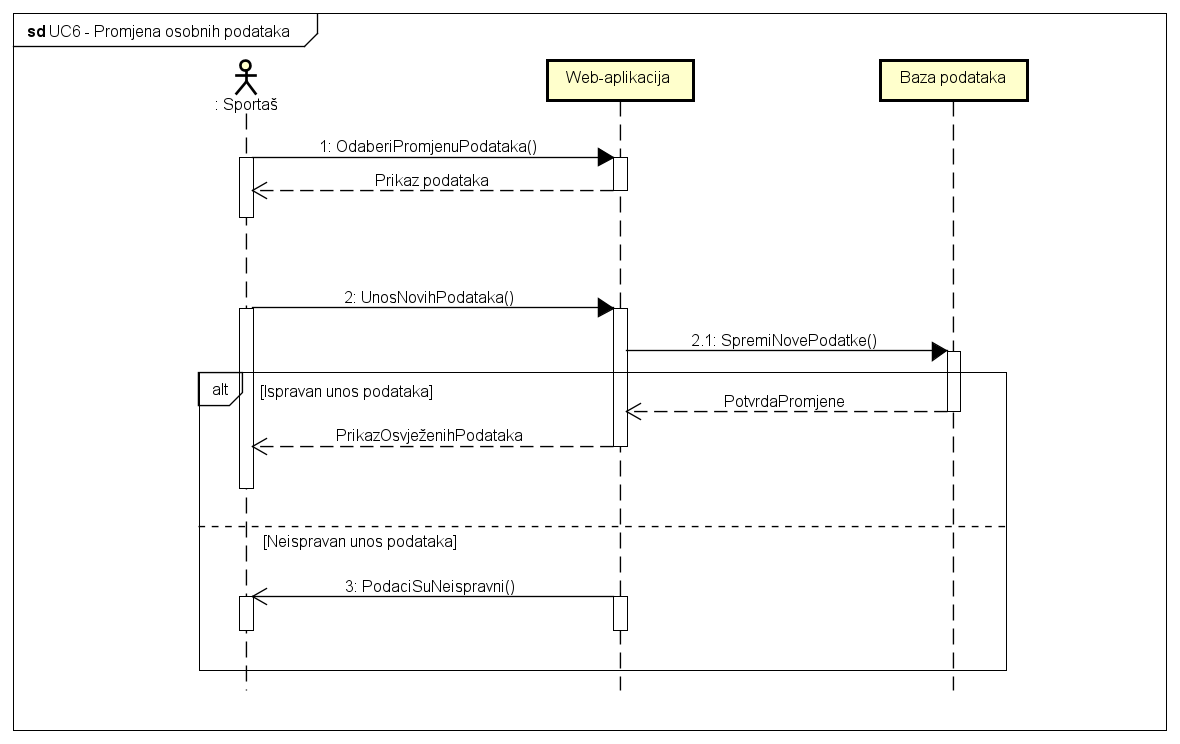
\includegraphics[width=\textwidth]{slike/UC6_SEKV_DIJ.png}
					\caption{Sekvencijski dijagram za UC6}
				\end{figure}
			
				\subsubsection{Obrazac uporabe UC7 - Prijava na sportsku aktivnost}
				Prijavljeni korisnik šalje zahtjev za odabir željene sportske aktivnosti. Poslužitelj zatim prikazuje kartu na kojoj se nalaze sve lokacije na kojima se održava sportska aktivnost koju je korisnik odabrao i koje imaju slobodnih mjesta. Korisnik zatim odabire željenu lokaciju i prijavljuje se za aktivnost. Poslužitelj zatim sprema prijavu u bazu podataka. Nakon što poslužitelj dobije potvrdu od baze da su podaci spremljeni, preusmjerava korisnika na stranicu gdje se nalaze sve prijavljene korisnikove aktivnosti. 
				
				\begin{figure}[H]
					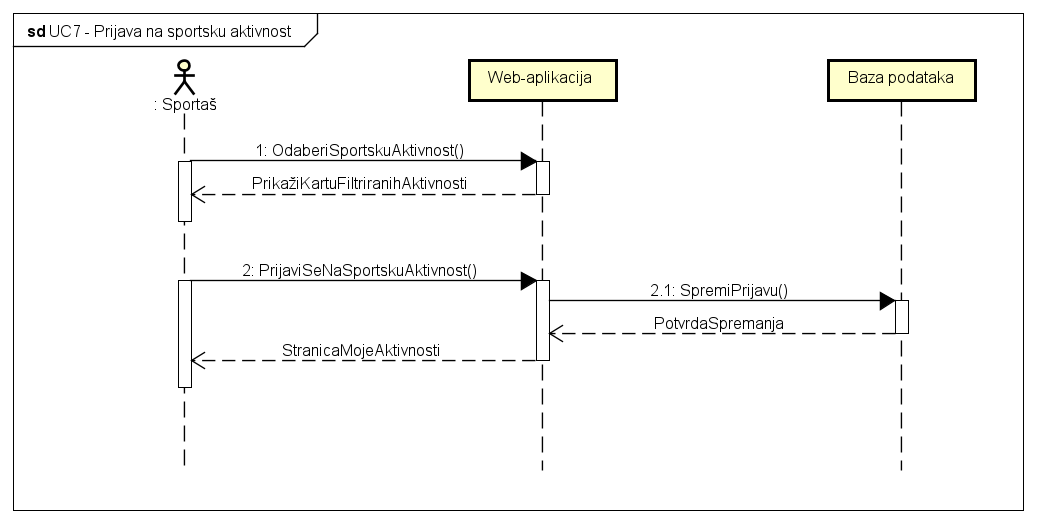
\includegraphics[width=\textwidth]{slike/UC7_SEKV_DIJ.png}
					\caption{Sekvencijski dijagram za UC7}
				\end{figure}
			
				\subsubsection{Obrazac uporabe UC10 - Iznajmljivanje sportskih površina/dvorana}
				Prilikom organiziranja sportske aktivnosti prijavljeni korisnik šalje zahtjev za iznajmljivanje sportske površine/dvorane. Poslužitelj zatim prikazuje dostupne sportske površina/dvorana koje se mogu iznajmiti. Prijavljeni korisnik zatim odabire željenu sportsku površinu/dvoranu. Nakon toga prijavljeni korisnik odabire željeni datum. Poslužitelj zatim provjerava u bazi postoje li slobodni termini na datum koji je korisnik izabrao. Ako oni ne postoje, obaviještava se korisnika da odabere neki drugi datum. Ako postoje slobodni termini na odabrani datum poslužitelj ih prikazuje prijavljenom korisniku. Korisnik zatim odabire željeni termin i nakon toga šalje zahtjev za potvrdu rezervacije. Poslužitelj sprema rezervaciju u bazu podataka i nakon što dobije potvrdu da je rezervacija spremljena o tome obaviještava korisnika.
				
				\begin{figure}[H]
					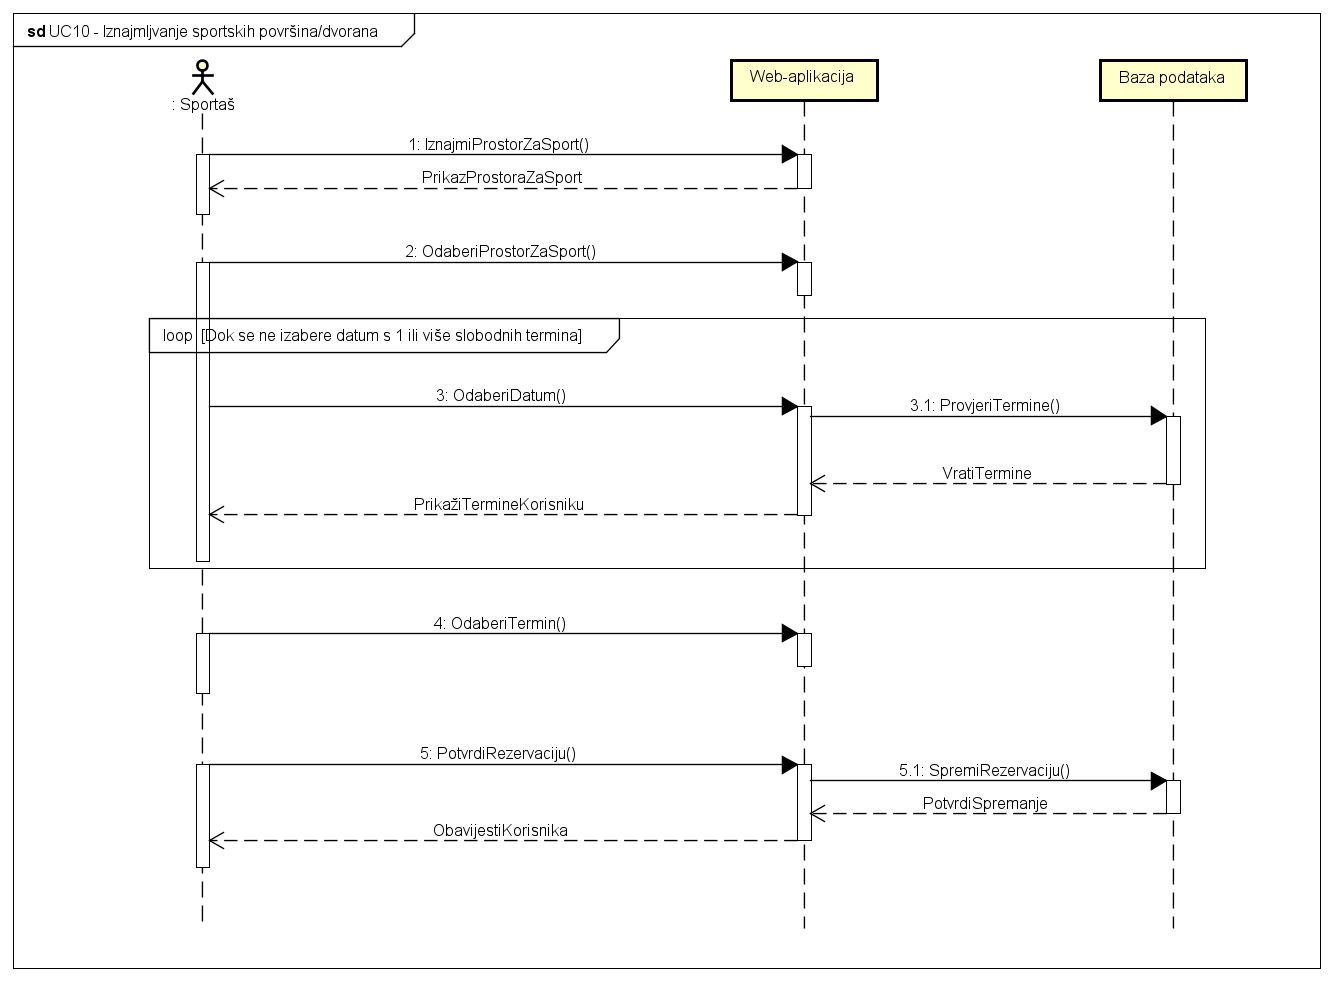
\includegraphics[width=\textwidth]{slike/UC10_SEKV_DIJ.png}
					\caption{Sekvencijski dijagram za UC10}
				\end{figure}
			
				\subsubsection{Obrazac uporabe UC21 - Prilaganje službene dokumentacije}
				Prijavljeni korisnik šalje zahtjev za dodavanje službene dokumentacije. Poslužitelj prikazuje obrazac za prijavu dokumentacije. Prijavljeni korisnik zatim unosi svoje podatke, te ako su oni ispravni poslužitelj ih sprema u bazu podataka. Nakon što baza podataka spremi podatke, vraća potvrdu poslužitelju koji zatim preusmjerava prijavljenog korisnika na stranicu kojom se korisniku daje do znanja da je njegova prijava zaprimljena te da će biti obaviješten kada ona bude obrađena. Administrator zatim može zatražiti pregled svih dokumentacija iz baze podataka i pregledati nove prijave. Ako su svi podaci ispravni administrator potvrđuje dokumentaciju i potvrđenu dokumentaciju sprema u bazu podataka. Ako su podaci neispravni prijava se briše iz baze podataka. Zatim administrator osvježi stanje prijave na poslužitelju, a nakon toga poslužitelj obaviještava korisnika o stanju njegove prijave. Ako su podaci bili neispravni kod samog upisa poslužitelj odmah javlja grešku korisniku.
				
				\begin{figure}[H]
					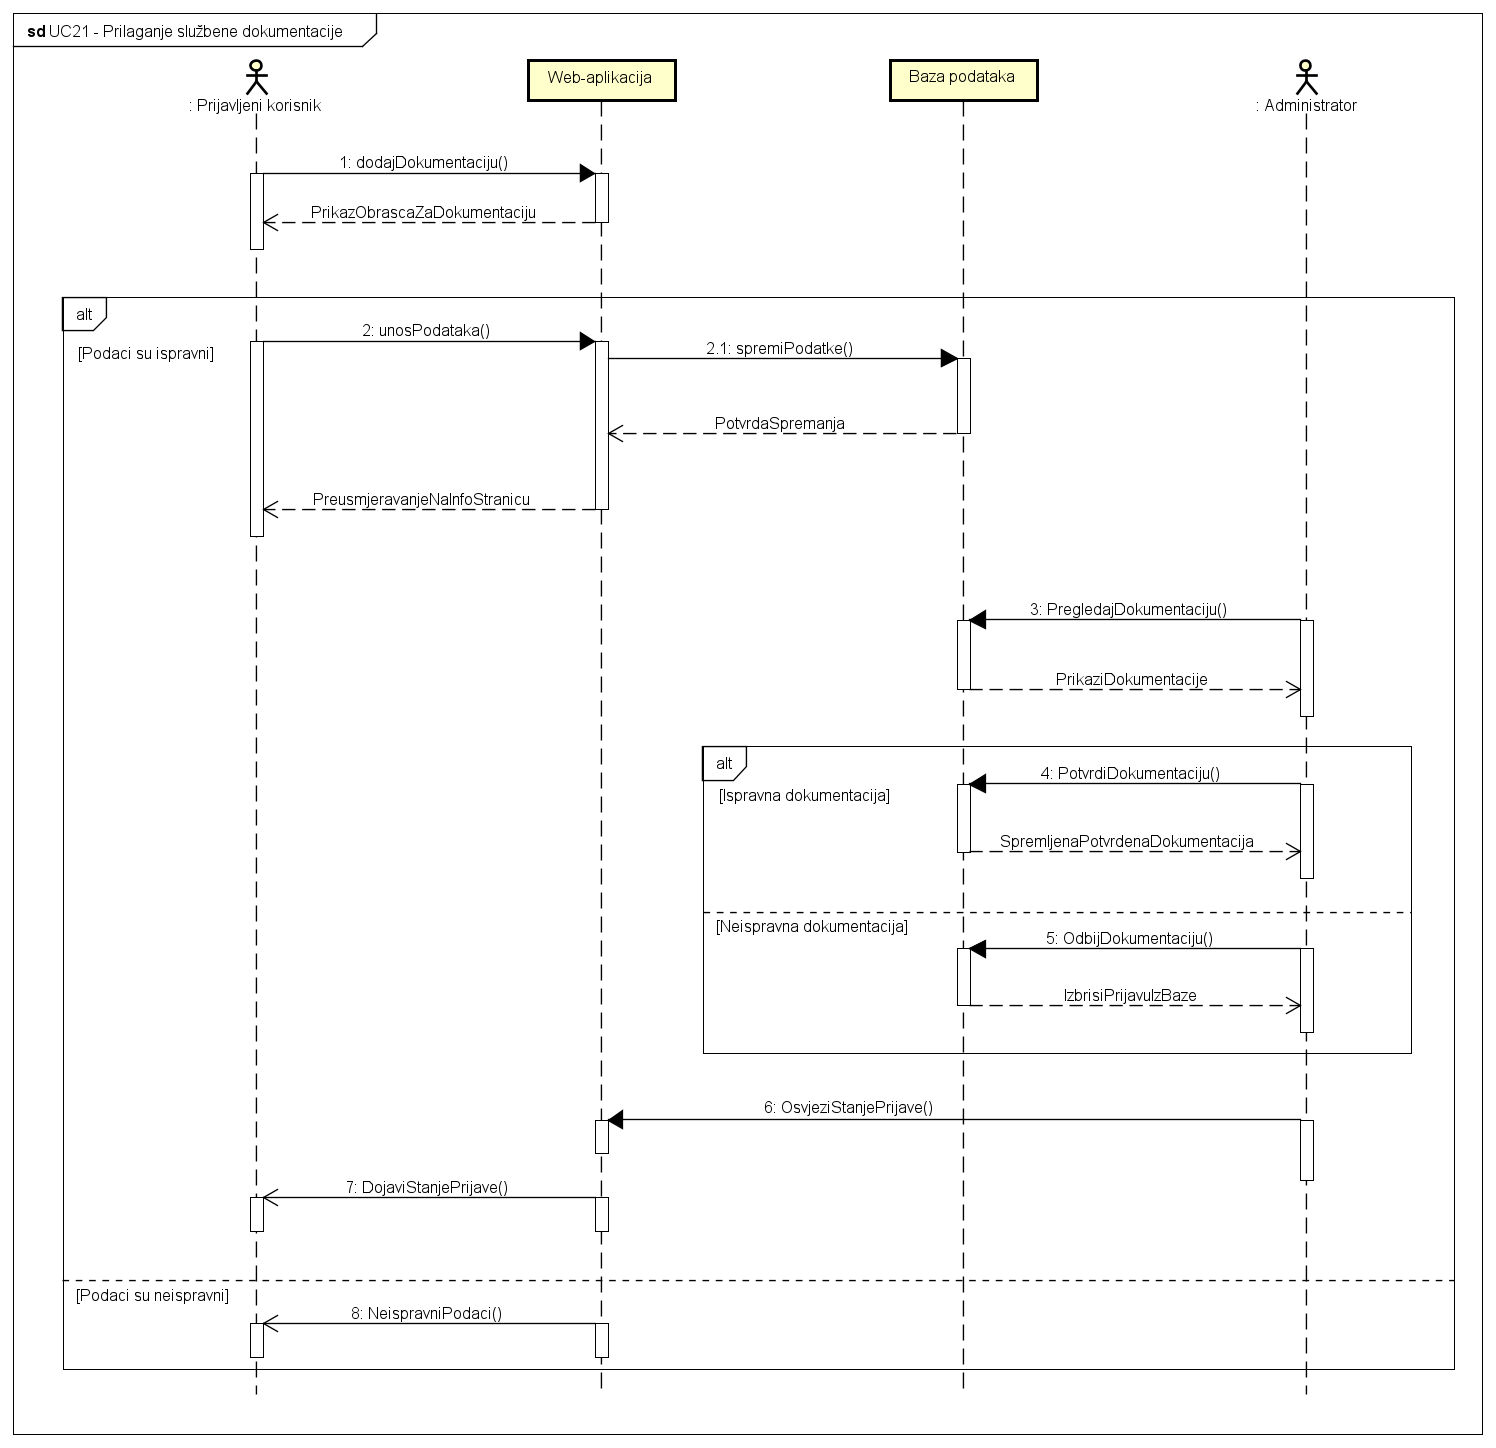
\includegraphics[width=\textwidth]{slike/UC21_SEKV_DIJ.png}
					\caption{Sekvencijski dijagram za UC21 }
				\end{figure}
		\eject
		\section{Ostali zahtjevi}
		
			\begin{comment}
			\textbf{\textit{dio 1. revizije}}\\
		 
			 \textit{Nefunkcionalni zahtjevi i zahtjevi domene primjene dopunjuju funkcionalne zahtjeve. Oni opisuju \textbf{kako se sustav treba ponašati} i koja \textbf{ograničenja} treba poštivati (performanse, korisničko iskustvo, pouzdanost, standardi kvalitete, sigurnost...). Primjeri takvih zahtjeva u Vašem projektu mogu biti: podržani jezici korisničkog sučelja, vrijeme odziva, najveći mogući podržani broj korisnika, podržane web/mobilne platforme, razina zaštite (protokoli komunikacije, kriptiranje...)... Svaki takav zahtjev potrebno je navesti u jednoj ili dvije rečenice.}
			\end{comment}
			
			\begin{itemize}
				\setlength{\itemsep}{0pt}
				\setlength{\parskip}{0pt}
				\item Sustav treba biti implementiran kao web aplikacija koristeći objektno-orijentirane jezike
				\item Pristup bazi podataka mora biti zaštićen i ne smije trajati duže od nekoliko sekundi
				\item Sustav mora podržavati hrvatsku abecedu uključujući dijakritičke znakove
				\item Sustavu istovremeno mogu pristupiti više različitih vrsta korisnika
				\item Korisničko sučelje mora biti jednostavno, responzivno i intuitivno za korištenje te se mora ispravno prikazivati na stolnim računalima, laptopima i mobilnim uređajima
				\item Neispravno korištenje korisničkog sučelja ne smije narušiti funkcionalnosti sustava
				\item Nadogradnja sustava ne smije narušiti funkcionalnosti sustava
				\item Sustav mora prijavljenim korisnicima jasno prikazati ovlasti koje im pripadaju (sportaš, trener, iznajmljivač)
				\item Sustav kao valutu za prikaz cijena i transakcija koristi HRK
				\item Pristup sustavu se mora odvijati pomoću protokola HTTPS
			\end{itemize}
			
			 
			 
			 
	